\documentclass[10pt, conference]{IEEEtran}
\usepackage[utf8]{inputenc}
\usepackage{amsmath,amssymb,amsfonts}
\usepackage{graphicx}
\usepackage{booktabs}
\usepackage{hyperref}
\usepackage{cite}
\usepackage[font=small,labelfont=bf]{caption}

\hypersetup{
    colorlinks=true,
    linkcolor=blue,
    filecolor=magenta,      
    urlcolor=cyan,
    pdftitle={Object Detection using DETR},
    pdfpagemode=FullScreen,
}

% Paper title
\title{Object Detection Using DETR}

% Author names
\author{
\IEEEauthorblockN{Kodavali Purnendra Sri Krishnaditya}
\IEEEauthorblockA{23125017}
\and
\IEEEauthorblockN{Gunta Preetham}
\IEEEauthorblockA{23125013}


}

\begin{document}

\maketitle

% ABSTRACT 
\begin{abstract}
This report details the implementation and evaluation of the Detection Transformer (DETR) model for object detection on a custom dataset of traffic scenes. DETR represents a paradigm shift in object detection, eliminating the need for hand-designed components like Non-Maximum Suppression (NMS) and anchor generation by framing the task as a direct set prediction problem. We fine-tuned a pre-trained DETR model with a ResNet-50 backbone on a dataset of approximately 31,000 images, targeting 12 distinct object classes. Due to significant computational constraints, the model could not be trained to the extent suggested by standard practice. Despite incomplete convergence, the model achieved a moderate mean Average Precision (mAP) of 0.4233 at an IoU threshold of 0.50. Our evaluation reveals strong performance on large, common classes such as "Car" and "Truck" but highlights significant challenges in detecting small objects and differentiating between visually similar, fine-grained classes like various traffic light states. This work provides a practical analysis of DETR's performance under limited computational resources and offers insights into its strengths and weaknesses on a real-world custom dataset.
\end{abstract}

\begin{IEEEkeywords}
Object Detection, DETR, Transformers, Computer Vision, Deep Learning, Transfer Learning.
\end{IEEEkeywords}

\IEEEpeerreviewmaketitle

% INTRODUCTION 
\section{Introduction}
Object detection, a fundamental task in computer vision, has traditionally relied on complex pipelines involving region proposals, anchor boxes, and post-processing steps like Non-Maximum Suppression (NMS). While models like YOLO and R-CNN variants have achieved state-of-the-art performance, their architectures often include hand-designed components that can be intricate and difficult to tune.

The DETR (DEtection TRansformer) model, introduced by Carion et al. \cite{carion2020end}, offers a novel, end-to-end approach that simplifies this pipeline. By leveraging a transformer-based encoder-decoder architecture, DETR treats object detection as a direct set prediction problem. It eliminates the need for anchors and NMS by producing a fixed-size set of predictions, which are matched to ground truth objects using a bipartite matching algorithm. This direct, set-based objective function enforces unique predictions per object.

This project aims to implement and evaluate a DETR model on a custom traffic scene dataset. We outline the full methodology, from data preprocessing and model fine-tuning to a comprehensive quantitative and qualitative evaluation of the results.

% METHODOLOGY 
\section{Methodology}

\subsection{Dataset and Preprocessing}
The initial dataset comprised a large collection of traffic scene images. A crucial first step was data cleaning; images without annotations or with clearly improper annotations were excluded from the dataset. This resulted in a final set of approximately 31,000 viable images. The data was partitioned into training, validation, and test sets with a 75\%, 10\%, and 15\% split, respectively.

The DETR architecture requires annotations in the COCO format. As our initial dataset used YOLO-style annotations (class index and normalized bounding box coordinates: \texttt{[x\_center, y\_center, width, height]}), a conversion script was implemented to transform them into the COCO format, which specifies bounding boxes as \texttt{[x\_min, y\_min, width, height]}.

\subsection{DETR Model Architecture}
The DETR model consists of three main components: a CNN backbone for feature extraction, a transformer encoder-decoder, and a feed-forward network (FFN) for final predictions.

\subsubsection{Backbone}
We used a ResNet-50 model, pre-trained on ImageNet, as the CNN backbone. It extracts a lower-resolution feature map from the input image, which is then passed to the transformer.

\subsubsection{Transformer and Set Prediction}
The core of DETR is its transformer architecture. The encoder refines the image features using self-attention, while the decoder takes a fixed number of learned positional embeddings, referred to as "object queries," and cross-attends to the encoder's output to generate object-specific embeddings. Each of these output embeddings is then passed to two parallel FFNs: one for class prediction (including a "no object" class) and one for bounding box prediction.

\subsubsection{Bipartite Matching Loss}
The core innovation of DETR is its set-based loss function, which enforces unique predictions for each object. This process involves two stages: first, finding an optimal one-to-one matching between the model's predictions and the ground truth objects, and second, computing the loss for the matched pairs.

Let $y$ be the set of ground truth objects, padded with $\emptyset$ (no object) to a fixed size $N$. Let $\hat{y} = \{\hat{y}_i\}_{i=1}^N$ be the set of $N$ predictions. Each prediction $\hat{y}_i$ consists of a class probability distribution $\hat{p}_i(c)$ and a predicted bounding box $\hat{b}_i$.

\paragraph{1. Optimal Assignment ($\hat{\sigma}$)}
The model must find the optimal permutation $\hat{\sigma} \in \mathfrak{S}_N$ that pairs predictions to ground truths by minimizing a total matching cost. This is an assignment problem solved efficiently with the Hungarian algorithm.
\begin{equation}
\hat{\sigma} = \underset{\sigma \in \mathfrak{S}_N}{\arg\min} \sum_{i=1}^{N} \mathcal{L}_{\text{match}}(y_i, \hat{y}_{\sigma(i)})
\label{eq:sigma_hat}
\end{equation}
Here, $\mathcal{L}_{\text{match}}$ is the pair-wise matching cost between a ground truth $y_i$ and a prediction with index $\sigma(i)$.

\paragraph{2. Pair-wise Matching Cost ($\mathcal{L}_{\text{match}}$)}
The cost used to find the optimal assignment considers both class prediction and bounding box similarity. For a ground truth $y_i=(c_i, b_i)$, where $c_i$ is the class label and $b_i$ is the box, the matching cost is defined as:
\begin{equation}
\mathcal{L}_{\text{match}}(y_i, \hat{y}_{\sigma(i)}) = \mathbf{1}_{\{c_i \neq \emptyset\}} \left[ -\hat{p}_{\sigma(i)}(c_i) + \mathcal{L}_{\text{box}}(b_i, \hat{b}_{\sigma(i)}) \right]
\label{eq:l_match}
\end{equation}
The indicator function $\mathbf{1}_{\{c_i \neq \emptyset\}}$ ensures that the cost is only computed for actual objects, not the padded $\emptyset$ slots. The cost encourages pairing predictions that are confident about the correct class (term $-\hat{p}_{\sigma(i)}(c_i)$) and have a small box localization error (term $\mathcal{L}_{\text{box}}$).

\paragraph{3. Bounding Box Loss ($\mathcal{L}_{\text{box}}$)}
The box loss, used in both the matching cost and the final loss, is a linear combination of the L1 loss and the Generalized Intersection over Union (GIoU) loss.
\begin{equation}
\mathcal{L}_{\text{box}}(b, \hat{b}) = \lambda_{\text{iou}}\mathcal{L}_{\text{GIoU}}(b, \hat{b}) + \lambda_{\text{L1}}\|b - \hat{b}\|_1
\label{eq:l_box}
\end{equation}
Here, $\lambda_{\text{iou}}$ and $\lambda_{\text{L1}}$ are hyperparameters that balance the two loss terms. The L1 loss provides scale-sensitivity, while the GIoU loss addresses the weaknesses of standard IoU.

\paragraph{4. Generalized IoU Loss ($\mathcal{L}_{\text{GIoU}}$)}
The GIoU loss is used to provide a meaningful gradient even when boxes do not overlap. It is defined as:
\begin{equation}
\mathcal{L}_{\text{GIoU}}(b, \hat{b}) = 1 - \left( \text{IoU}(b, \hat{b}) - \frac{|C \setminus (b \cup \hat{b})|}{|C|} \right)
\label{eq:l_giou}
\end{equation}
where $C$ is the smallest convex shape enclosing both the predicted box $\hat{b}$ and the ground truth box $b$. Unlike IoU, which is 0 for non-overlapping boxes, GIoU provides a non-zero loss that pushes the boxes towards each other.

\paragraph{5. Hungarian Loss ($\mathcal{L}_{\text{Hungarian}}$)}
After finding the optimal assignment $\hat{\sigma}$ using Eq.~\eqref{eq:sigma_hat}, the final loss is computed as a sum over all matched pairs. This is the loss that is backpropagated to train the model.
\begin{align}
\mathcal{L}_{\text{Hungarian}}(y, \hat{y}) = \sum_{i=1}^{N} \bigg[ &-\log \hat{p}_{\hat{\sigma}(i)}(c_i) \nonumber \\
& + \mathbf{1}_{\{c_i \neq \emptyset\}} \mathcal{L}_{\text{box}}(b_i, \hat{b}_{\hat{\sigma}(i)}) \bigg]
\label{eq:l_hungarian}
\end{align}
This loss combines a negative log-likelihood for class prediction (similar to cross-entropy) and the $\mathcal{L}_{\text{box}}$ for the bounding boxes. The class loss is computed for all pairs, including the "no object" class, while the box loss is only computed for pairs corresponding to actual objects.

\subsection{Model Training}
We utilized a pre-trained DETR model from the Hugging Face `transformers` library, which comes with a ResNet-50 backbone pre-trained on ImageNet. The final classification head was replaced with a new one configured for our 12 distinct object classes.

To accelerate training and leverage learned features, we employed a fine-tuning strategy. The parameters of the entire ResNet-50 backbone were frozen. This meant that only the transformer encoder, decoder, and the final prediction heads were updated during training, reducing the number of trainable parameters to approximately 18 million (43.5\% of the total parameters).

Training was conducted on a single NVIDIA P100 GPU provided by the Kaggle platform. Training DETR is notoriously slow to converge. The original paper reports a 300-epoch baseline schedule requiring $\sim$6 days on 8 V100 GPUs \cite{carion2020end}. In our setup, a single epoch on our dataset took approximately 1.5 hours. Due to platform time limits, we were only able to train the model for 38 epochs, totaling approximately 52 hours. This limited training duration meant the model did not fully converge, which is a critical factor in interpreting the final evaluation results.

% EVALUATION AND RESULTS
\section{Evaluation and Results}

\subsection{Mean Average Precision (mAP)}
The model's overall performance was evaluated using the standard COCO evaluation metrics. The primary metric, mAP@0.50, reached 0.4233, indicating a moderate level of performance. A breakdown by object size reveals a significant weakness in detecting small objects.

\begin{table}[h!]
\centering
\caption{Overall Mean Average Precision (mAP) Metrics}
\label{tab:map_overall}
\begin{tabular}{@{}lc@{}}
\toprule
\textbf{Metric} & \textbf{Value} \\ \midrule
\textbf{map\_50 (IoU=0.50)} & \textbf{0.4233} \\
map\_small          & 0.0635 \\
map\_medium         & 0.2595 \\
map\_large          & 0.4052 \\ \bottomrule
\end{tabular}
\end{table}

The low \texttt{map\_small} value of 0.0635 suggests the model struggles to resolve fine-grained details or that there was a lack of high-quality labels for small objects in the training set. Performance clearly improves with object size, as seen in the \texttt{map\_large} score of 0.4052.

\subsection{Per-Class Analysis}
We further analyzed performance on a per-class basis. Table~\ref{tab:map_class} shows the mAP for each of the 12 classes, while Table~\ref{tab:pr_f1} provides the corresponding precision, recall, and F1-scores. The data from these tables is visualized in Figure~\ref{fig:map_per_class} and Figure~\ref{fig:prf1_per_class} for easier comparison.

\begin{table}[h!]
\centering
\caption{Mean Average Precision (mAP@0.50) per Class}
\label{tab:map_class}
\begin{tabular}{@{}clc@{}}
\toprule
\textbf{Class ID} & \textbf{Class Name} & \textbf{mAP per Class} \\ \midrule
11 & truck & 0.3930 \\
2 & car & 0.3587 \\
1 & biker & 0.3105 \\
4 & traffic light & 0.2792 \\
7 & traffic light-red & 0.2655 \\
3 & pedestrian & 0.2142 \\
12 & arret & 0.1914 \\
9 & traffic light-yellow & 0.1605 \\
10 & traffic light-yellow left & 0.1448 \\
8 & traffic light-red left & 0.1403 \\
5 & traffic light-green & 0.0776 \\
6 & traffic light-green left & 0.0426 \\ \bottomrule
\end{tabular}
\end{table}

\begin{table}[h!]
\centering
\caption{Precision, Recall, and F1-Score per Class}
\label{tab:pr_f1}
\begin{tabular}{@{}lccc@{}}
\toprule
\textbf{Class Name} & \textbf{Precision} & \textbf{Recall} & \textbf{F1 Score} \\ \midrule
truck & 0.5256 & 0.7303 & 0.6113 \\
car & 0.4695 & 0.7459 & 0.5763 \\
traffic light & 0.4009 & 0.6835 & 0.5054 \\
biker & 0.4188 & 0.6490 & 0.5091 \\
traffic light-red & 0.4009 & 0.6487 & 0.4955 \\
pedestrian & 0.3379 & 0.6301 & 0.4399 \\
arret & 0.3352 & 0.6000 & 0.4301 \\
traffic light-yellow & 0.2717 & 0.4694 & 0.3442 \\
traffic light-red left & 0.2567 & 0.4253 & 0.3201 \\
traffic light-green & 0.1880 & 0.3758 & 0.2506 \\
traffic light-yellow left & 0.1826 & 0.3643 & 0.2433 \\
traffic light-green left & 0.0757 & 0.1812 & 0.1067 \\ \midrule
\textbf{Micro-Average} & \textbf{0.4038} & \textbf{0.6730} & \textbf{0.5048} \\ \bottomrule
\end{tabular}
\end{table}

The results show a clear hierarchy in performance. "Truck" and "Car" are the best-performing classes, likely due to their large size, distinct features, and high frequency in the dataset. Conversely, fine-grained traffic light states, such as "traffic light-green left", perform very poorly. This can be attributed to a combination of factors: small object size, high visual similarity between classes, and potentially fewer training examples.

A consistent trend across many classes is that recall is significantly higher than precision. The micro-averaged recall of 0.6730 versus a precision of 0.4038 indicates a global tendency for the model to produce more false positives than false negatives. It is effective at finding objects but often misclassifies them or detects non-existent objects.

\begin{figure}[htbp]
    \centering
    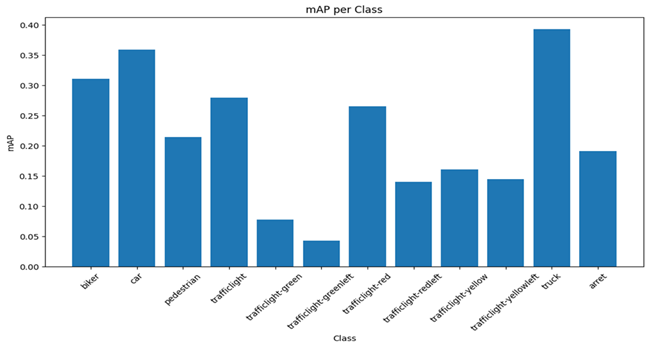
\includegraphics[width=\linewidth]{images/map_per_class.png}
    \caption{Visual comparison of Mean Average Precision (mAP@0.50) across all 12 classes. This chart visualizes the data presented in Table~\ref{tab:map_class}, highlighting the superior performance on classes like "Truck" and "Car" and the significant challenge in detecting specific traffic light states.}
    \label{fig:map_per_class}
\end{figure}

\begin{figure}[htbp]
    \centering
    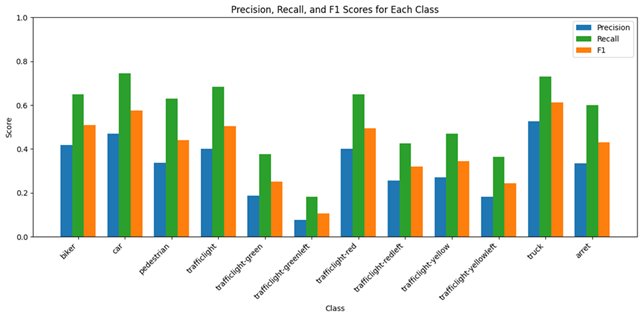
\includegraphics[width=\linewidth]{images/precision_recall_f1_perclass.png}
    \caption{Per-class Precision, Recall, and F1-scores. This visualization corresponds to the metrics in Table~\ref{tab:pr_f1}. The generally higher recall compared to precision is evident across most classes, indicating a tendency for more false positives.}
    \label{fig:prf1_per_class}
\end{figure}

\subsection{Confusion Matrix}
The confusion matrix (Fig. \ref{fig:confusion_matrix}) provides a visual representation of class-wise errors. The diagonal represents correct classifications, while off-diagonal cells show misclassifications. We observe confusion between different states of traffic lights, which aligns with the poor per-class metrics for these categories.

\begin{figure}[h!]
    \centering
    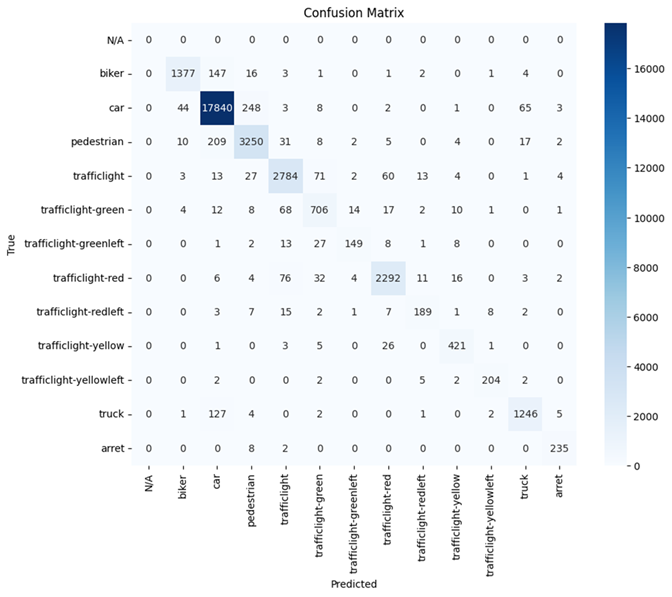
\includegraphics[width=0.9\linewidth]{images/confusion_matrix.png}
    \caption{Confusion matrix visualizing class-wise prediction accuracy. Values on the diagonal represent true positives, while off-diagonal cells indicate misclassifications.}
    \label{fig:confusion_matrix}
\end{figure}

\subsection{Localization Accuracy}
The Intersection over Union (IoU) distribution histogram for true positive predictions is shown in Fig. \ref{fig:iou_hist}. The histogram is strongly skewed to the right, with a majority of true positives achieving an IoU between 0.7 and 0.9. This is a positive indicator, suggesting that when the model correctly detects and classifies an object, its bounding box localization is generally accurate.

\begin{figure}[h!]
    \centering
    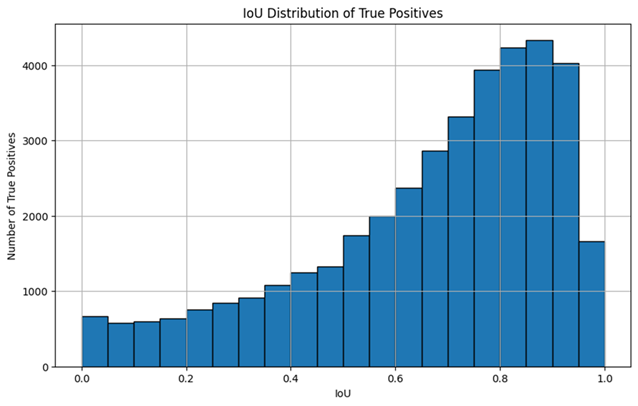
\includegraphics[width=0.9\linewidth]{images/iou_distribution.png}
    \caption{IoU distribution histogram for true positive predictions. The high concentration of IoUs > 0.7 indicates accurate bounding box localization for correctly classified objects.}
    \label{fig:iou_hist}
\end{figure}


% QUALITATIVE RESULTS 
\section{Qualitative Results}
Qualitative analysis of predictions on test images (Fig. \ref{fig:predictions}) corroborates the quantitative findings. The model reliably detects large objects like cars and trucks with well-fitted bounding boxes. However, smaller and more distant objects, such as pedestrians or traffic lights, are often missed or incorrectly classified, highlighting the challenges identified in our metric-based evaluation.

\begin{figure}[h]
    \centering
    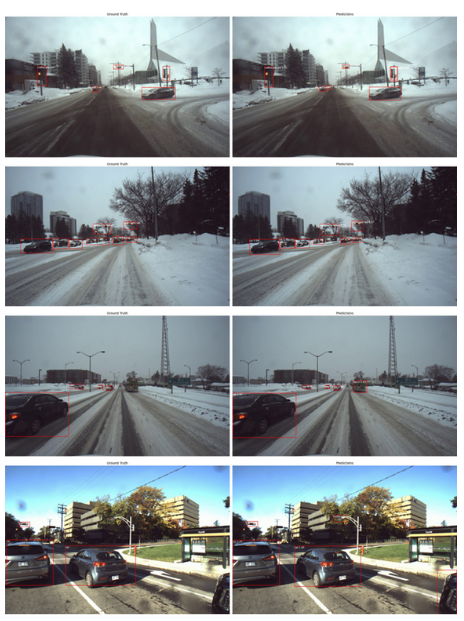
\includegraphics[width=0.9\linewidth]{images/predictions.png}
    \caption{Example predictions on test set images. The model demonstrates proficiency in detecting prominent objects like cars but struggles with smaller, distant, or fine-grained objects.}
    \label{fig:predictions}
\end{figure}
 

% CONCLUSION 
\section{Conclusion}
In this project, we successfully implemented and fine-tuned a DETR model for object detection on a custom dataset. Despite significant limitations in computational resources and training time, which prevented the model from fully converging, we achieved a moderate overall mAP@0.50 of 0.4233.

Our evaluation demonstrated that the model performs well on large, distinct classes like "Car" and "Truck", and provides accurate bounding box localization for its correct predictions. However, its performance degrades substantially for small objects and for classes requiring fine-grained distinction, such as different traffic light states. The model's tendency for high recall at the cost of lower precision suggests that with further training, it could learn to better discriminate between true and false positives.

Future work should prioritize training for the full 300-epoch schedule to allow for proper convergence. Additionally, techniques like data augmentation specifically targeting small objects, or employing a more advanced backbone like Swin Transformer, could help address the identified weaknesses and unlock the full potential of the end-to-end DETR framework.

% REFERENCES 
\bibliographystyle{IEEEtran}
\bibliography{refs}

\end{document}